\documentclass[10pt]{article}
\usepackage[a4paper,margin=2.3cm]{geometry}
\usepackage[T1]{fontenc}
\usepackage{microtype}
\usepackage{amsmath}
\usepackage{txfonts}
\usepackage{bm}
\usepackage{graphicx,booktabs,tabularx,multirow,xcolor,enumitem,caption,subcaption}
\usepackage[numbers,sort&compress]{natbib}
\usepackage[colorlinks=true,linkcolor=blue!50!black,citecolor=blue!50!black,urlcolor=blue!50!black]{hyperref}
\captionsetup{font=small,labelfont=bf}
\setlist{nosep,leftmargin=*}
\newcommand{\pass}{\textcolor{green!45!black}{\textbf{pass}}}
\newcommand{\fail}{\textcolor{red!70!black}{\textbf{fail}}}
\newcommand{\Dk}{D(k)}
\newcommand{\E}{\mathbb{E}}

\title{\textbf{The training split chooses the circuit:}\\[2pt]
\large Predicting and steering which Fourier frequencies a grokking network learns}
\author{Seungho Yu \and Claude (Anthropic)\thanks{Claude (model \texttt{claude-opus-5-5}) is an AI system. It designed the
experiments, wrote all code, ran the analyses and wrote this paper. Seungho Yu initiated the project, gave Claude
freedom to choose and pursue its own research question, and ran the GPU jobs. See the contribution statement in
Section~\ref{sec:contrib}. Code, data and pre-registrations: \url{https://github.com/yuseunghogi-commits/grokking-frequency-selection} (currently private).}}
\date{October 2026 \quad (preprint, not peer reviewed)}

\begin{document}
\maketitle

\begin{abstract}
\noindent
Transformers trained on modular addition with weight decay eventually \emph{grok}. They represent numbers as rotations
at a handful of key Fourier frequencies, and which frequencies a run uses has been described as seed-dependent. We ask
whether the frequencies can be predicted, and chosen, before training. In a pre-registered init~$\times$~split factorial
on held-out seeds, the frequencies that lead early are set jointly by the initialisation \emph{and} by which 30\,\% of
the equations are in the training set. Together the two predict 1265 of 3072 top-3 slots, against 655 for the init
alone, 959 for the data alone and 165 by chance. The data effect is collective and algebraic: it survives relabelling
$a\mapsto a{+}t$ and disappears when the labels are shuffled. We give a training-free statistic for it, the Fourier power
\Dk\ of the \emph{shared-answer} matrix $N[a,a']$, which counts the answers $c$ that inputs $a$ and $a'$ share in the
training set. \Dk\ predicts the data effect on unseen splits (pre-registered $\rho=0.71$). It also does so at other primes,
for multiplication (in the discrete-log basis) and in a two-layer model ($\rho=0.65$--$0.74$). Used in reverse, \Dk\
becomes a control: by swapping about 12\,\% of the training pairs to maximise \Dk\ for a randomly chosen target frequency,
with the numbers of pairs per input and per answer unchanged, we make the target a key frequency of the final circuit in
\textbf{16/16} one-layer runs (vs.\ 1/16 on the original splits) and \textbf{15/16} two-layer runs (vs.\ 0/16), including
targets the initialisation disfavours. Two of our pre-registered theoretical predictions failed: a $\sqrt{1-f}$ law for how
the data effect weakens with the training fraction $f$, and an init-side readout for the two-layer model. We report both.
All results are for small models on modular arithmetic.
\end{abstract}

\section{Introduction}
Grokking~\citep{power2022grokking} is the sudden move from memorisation to generalisation long after the training set has
been fit. On modular addition it has a crisp mechanistic description~\citep{nanda2023progress}. The network embeds each
number $a$ as $\cos(\omega_k a),\sin(\omega_k a)$ for a few key frequencies $\omega_k = 2\pi k/p$ and computes
$\cos(\omega_k(a+b-c))$ through trigonometric identities (Fig.~\ref{fig:phen}). Which $k$ a run uses differs from run to
run~\citep{nanda2023progress,chughtai2023toy}. For MLPs, the initial embedding spectrum predicts which frequencies
survive~\citep{ding2024survival}, and lottery-ticket dynamics explain why~\citep{he2026mechanism}. Theory of the early
dynamics treats the finite training subset as zero-mean noise around the full table~\citep{wang2026probability}.

This paper asks a sharper question: \emph{given the initialisation and the training split, can we say before training
which frequencies the network will use, and can we choose them?} Our main findings are as follows.
\begin{enumerate}
\item \textbf{The split is not noise.} Holding the initialisation fixed, which pairs are in the training set shifts the
  favoured frequencies systematically, early (within $\sim$20 steps) and roughly additively with the init effect
  (Sec.~\ref{sec:factorial}).
\item \textbf{A closed form for the data side.} The data effect is cast by the algebraic structure of the equation set.
  It is predicted, without training, by the Fourier power \Dk\ of the shared-answer matrix (Sec.~\ref{sec:dk}). This
  holds across primes, for multiplication and in two layers (Sec.~\ref{sec:general}). \Dk\ is a short corollary of known
  early-gradient analyses~\citep{yao2025probability,wang2026probability,tian2025provable}, and we test it per frequency
  on finite splits.
\item \textbf{Steering.} Editing $\sim$12\,\% of the training pairs according to \Dk\ makes a pre-chosen frequency part of
  the final circuit in 31 of 32 fully trained runs across one- and two-layer models, against 1 of 32 on unedited splits
  (Sec.~\ref{sec:steer}).
\item \textbf{The init side, partly.} In one layer the operands reach the MLP only through the attention OV path. That
  explains why the OV spectrum at initialisation predicts the init effect better than the embedding spectrum, and the
  unembedding adds independent information. Our pre-registered extension of this argument to two layers failed
  (Sec.~\ref{sec:init}).
\end{enumerate}
Every confirmatory claim was pre-registered: hypotheses, thresholds and analysis were written down and hashed before the
runs existed. We report every outcome, including the failures (Table~\ref{tab:prereg}).

\begin{figure}[t]\centering
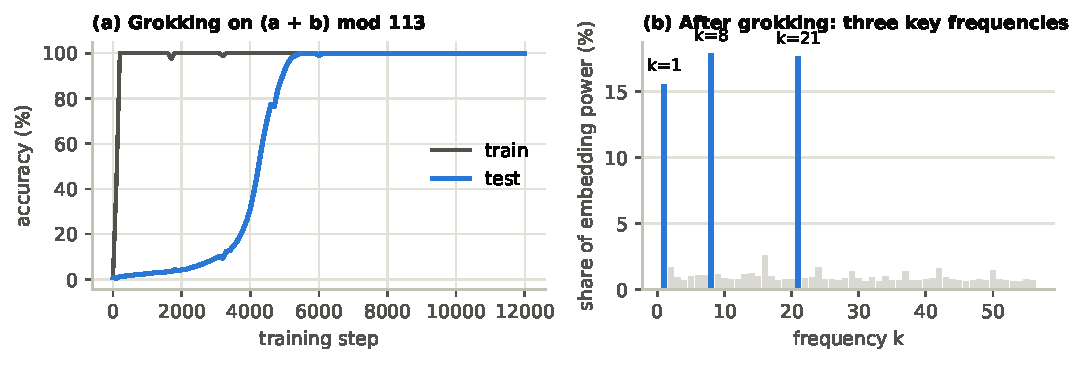
\includegraphics[width=\linewidth]{figures/fig1_phenomenon.pdf}
\caption{\textbf{The phenomenon.} (a)~A one-layer transformer on $(a+b)\bmod 113$, trained on 30\,\% of all pairs, fits
the training set within a few hundred steps and generalises around step 5000. (b)~After grokking, the embedding's Fourier
power is concentrated on three key frequencies ($k=1,8,21$ in this run), which carry 94\,\% of the embedding power.
Removing them from the MLP activations sends test accuracy to chance; keeping only them preserves it.}
\label{fig:phen}
\end{figure}

\section{Related work}
\label{sec:related}
\textbf{Mechanism and universality.} Modular-addition networks use sparse Fourier
features~\citep{nanda2023progress,gromov2023grokking}, with ``clock'' and ``pizza'' variants~\citep{zhong2023clock}, and
group operations more generally use irreducible representations~\citep{chughtai2023toy}. Max-margin analyses show that
wide networks use all frequencies on the full table~\citep{morwani2024feature}.
\textbf{Which frequencies, and why.} \citet{ding2024survival} predict frequency survival in MLPs from the initial
embedding spectrum (Pearson 0.85). \citet{he2026mechanism} give a lottery-ticket account on the full dataset. Our init-side
results extend this line to transformers through the OV path; our data-side results address a factor these works hold
fixed.
\textbf{Early dynamics.} The leading term of our derivation (Sec.~\ref{sec:why}) appears in probability-signature
analyses~\citep{yao2025probability,wang2026probability} and in the lazy stage of Li$_2$~\citep{tian2025provable}. Those
works either use the full table or treat the subset as zero-mean noise. Shared answers are the ``parallelograms'' of
\citet{liu2022effective}. Kernel views~\citep{kumar2024grokking,rubin2024grokking,mallinar2025emergence,tomas2026breaking}
and margin views~\citep{mohamadi2024why} explain when grokking happens rather than which $k$ is chosen.
\textbf{Data controls representation.} The closest work is \citet{ledoux2026order}. In a very sparse regime ($p=9973$,
0.3\,\% of pairs), the \emph{order} of minibatches sets the learned fundamental frequency, and training-set composition
reportedly does not matter. We train full-batch, so there is no order; we change \emph{composition}, choose an arbitrary
target and verify the final circuit. \citet{kumar2026flat} select readout frequencies from learned features during
training; this differs from predicting selection from data alone. We use per-pair datamodels~\citep{ilyas2022datamodels}
as one tool.

\section{Setup}
\label{sec:setup}
\textbf{Task and model.} Inputs are $(a,b,\texttt{=})$ with $a,b\in\mathbb{Z}_{113}$; the target is $(a+b)\bmod 113$. The
model is the one-layer transformer of~\citet{nanda2023progress}: $d=128$, 4 heads, $d_{\text{mlp}}=512$, ReLU, no LayerNorm,
untied embed and unembed, logits read at \texttt{=}. Training is full-batch AdamW (lr $10^{-3}$ with a 10-step linear
warm-up, $\beta=(0.9,0.98)$, weight decay 1.0) on a random 30\,\% of all $p^2$ pairs (3830 pairs). An \emph{init} is the
seed of the parameters; a \emph{split} is the seed of the train/test partition, and the two are varied independently. We
train many models in parallel with stacked weights. A custom optimiser reproduces \texttt{torch.optim.AdamW} exactly
(maximum spectral difference $10^{-5}$). Section~\ref{sec:steer} also uses a two-block model: block 1 has causal attention
and an MLP at all positions, block 2 attention and an MLP at \texttt{=}. Multiplication uses tokens $1..p{-}1$ and the
discrete-log basis, so the group is $\mathbb{Z}_{p-1}$.

\textbf{Readouts.} The \emph{spectrum} of a run at step $t$ is the share of the Fourier power of $W_E$ (over tokens) at each
frequency $k=1..\lfloor (n-1)/2\rfloor$. The \emph{winners} are the top-3 frequencies of the step-200 or step-500 spectrum.
The \emph{key frequencies} of a trained one-layer run are found by clustering MLP neurons by their dominant 2-D frequency
and keeping clusters with $\ge 3\,\%$ of the live neurons. These were validated causally (Fig.~\ref{fig:phen}). For two
layers we pre-registered a logit rule: frequencies holding $\ge 5\,\%$ of the logit energy in the
$\cos/\sin\,k(a+b-c)$ components. A development pilot showed that this rule separates cleanly (keys 7--68\,\%, others
$\le 2.1\,\%$), and that its keys were a subset of those found by the neuron rule.

\textbf{Votes.} In a grid of inits~$\times$~splits, let $Z_{i,s}$ be the $z$-scored log spectrum of cell $(i,s)$. The
\emph{init vote} of a cell averages $Z$ over the same init on other splits. The \emph{data vote} averages $Z$ over the same
split with other inits and, from v2 on, is centred across splits to remove components shared through common inits. This
centring was introduced after a development smoke test (not archived) showed a spurious agreement of about 0.98 between two
conditions that shared inits.

\textbf{Statistics.} We report top-3 hits $\sum_{\text{cells}}|\text{pred}_3\cap\text{win}_3|$ (chance $9/n_f$ per cell).
Nulls are cluster-aware permutations: in a development smoke test (not archived) a hypergeometric null gave $p\approx3\cdot10^{-5}$ where the cluster-aware null
gave $0.0085$.
Confidence intervals are paired bootstraps over inits and splits. Rank agreement is the mean within-split Spearman
correlation, with permutation $p$-values. Noise ceilings are Spearman--Brown split-half reliabilities.

\textbf{Pre-registration.} Each confirmatory stage (v1--v7) was written down with its thresholds and analysis code, and
hashed (SHA-256) before its runs. The hash is stored in the result file, and from v5 on the text was also pushed to
GitHub before the run. Development and test seeds are disjoint. Table~\ref{tab:runs} lists the stages.

\begin{table}[t]\centering\small
\caption{\textbf{Experimental stages.} All confirmatory stages were pre-registered. ``Kaggle'' = one NVIDIA T4.}
\label{tab:runs}
\begin{tabularx}{\linewidth}{@{}l l X l@{}}\toprule
stage & where & design & claims \\\midrule
pilot & CPU & single runs; seeds; weight-decay control & reproduction \\
v1 & Kaggle, 9.4\,h & dev and test factorials ($32\times32$, step 500); 64 full runs; $2\times1536$-run datamodels; MLP and subtraction variants & C1--C6, R1 \\
v2 & Kaggle, 2.8\,h & data vote under relabel / shuffle / subtraction / MLP; per-pair datamodels; time course & H1--H5 \\
v3 & CPU & 16 fresh splits $\times$ 16 fresh inits, 200 steps & P1, P2 (\Dk) \\
v4 & CPU & $p\in\{59,97\}$, $+$ and $\times$; 8 splits $\times$ 12 inits & G1, G2 \\
v5 & CPU + Kaggle & steering: 8 random targets $\times$ 5 strengths $\times$ 12 inits; 32 full runs & S1--S4 \\
v6 & CPU & training fraction 0.85 vs 0.3 & F1 \\
v7 & Kaggle & steering and init readout in a 2-layer model; 192 short + 32 full runs & T1--T5 \\\bottomrule
\end{tabularx}
\end{table}

\section{Results}

\subsection{Initialisation and split both decide, and their effects add}
\label{sec:factorial}
On a held-out $32\times32$ factorial (1024 cells; fresh inits and splits), we predicted each cell's step-500 winners from its init
vote, its data vote, and their sum (Fig.~\ref{fig:votes}a). The init vote alone gets 655 of 3072 top-3 slots and the data
vote alone 959; chance is 165. Their $z$-sum gets \textbf{1265}, and both bootstrap intervals of the improvement exclude
zero ($[499,716]$ over init, $[212,409]$ over data; C1 \pass). The data effect is causal. A ridge datamodel fitted on 1536
runs per split ranks training pairs by their effect on the split's favourite frequency $k^\star$. Removing the top 10\,\%
of pairs drives $z(k^\star)$ to $-0.71$ and $-1.01$ in the two tested splits, compared with $+1.19$ and $+1.30$ for random
10\,\% removals and $+3.86$ and $+3.47$ for removing the bottom 10\,\% (C3 \pass, Holm $p=0.0002$ for both).

The step-500 winners are a leading-frequency target, not the final circuit. They agree with the step-200 winners in 96\,\%
of slots, but contain only 56.5\,\% of the final key frequencies of 64 fully trained runs. This is below the
validity threshold of 75\,\% that the v1 analysis code fixed before the run (the threshold is in the code, not in the
registration text), so we treat early winners and final circuits as separate outcomes and test both from v5 on.

\begin{figure}[t]\centering
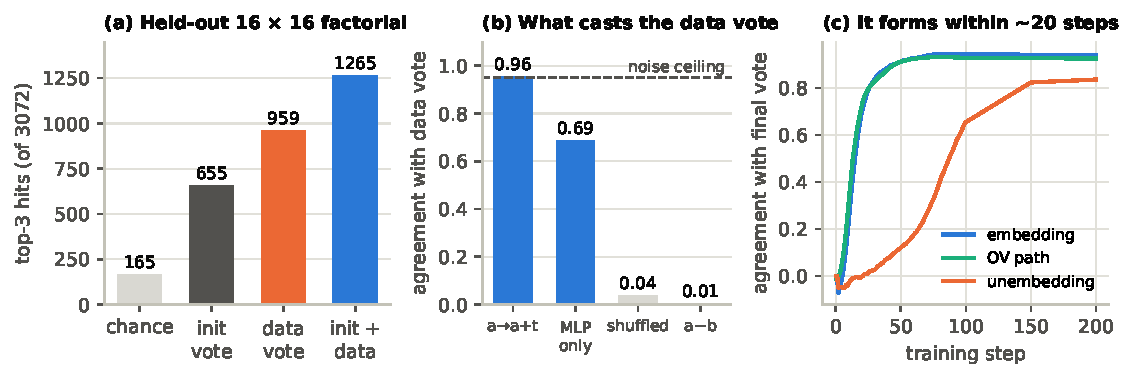
\includegraphics[width=\linewidth]{figures/fig3_votes.pdf}
\caption{\textbf{Two votes.} (a)~Top-3 hits on the held-out factorial (v1, pre-registered C1). (b)~Agreement of the data
vote in modified conditions with the true data vote on the same splits (v2). The dashed line is the noise ceiling. The
vote survives relabelling $a\mapsto a{+}t$ (0.96) and largely survives removing attention (MLP-only, 0.69). It vanishes
when the labels are shuffled (0.04) or the task is changed to subtraction on the same pairs (0.01). (c)~Time course: the
data vote appears in the embedding and the OV path within $\sim$20 steps; the unembedding lags behind.}
\label{fig:votes}
\end{figure}

\subsection{What casts the data vote}
\label{sec:anatomy}
Four pre-registered manipulations show what part of the data the vote comes from (Fig.~\ref{fig:votes}b; v2). Relabelling
every token $a\mapsto a+t$ changes every token identity but preserves which equations co-occur, and the vote is unchanged
(agreement 0.955, ceiling 0.957; H2 \pass). Shuffling the labels keeps the token statistics but destroys the group
structure, and the vote is gone (0.04). Training on $a-b$ with the same pairs gives an unrelated vote (0.006). An MLP-only
network on the same splits inherits most of the vote (0.69; H4 \pass), so the vote is largely a property of the data
rather than of attention. H5 asked whether per-pair influence (ridge datamodels on 1536 runs per split) is reproducible across two init groups
($\rho>0$, $p<0.01$ in at least 3 of 4 splits). Only 2 of 4 splits passed ($\rho=0.02$--$0.04$; H5 \fail), and the
datamodels predict held-out runs poorly ($R^2\approx0.03$, descriptive): the vote is spread over many equations, and no
small set of pairs carries it. The vote forms within the first $\sim$20 steps in the embedding and the OV path
(Fig.~\ref{fig:votes}c), long before grokking.

\subsection{A closed form for the data vote: shared answers}
\label{sec:dk}
Call two inputs $a,a'$ \emph{answer-sharing} if, for some $c$, both $(a,c-a)$ and $(a',c-a')$ are training equations.
Let $N[a,a']$ count such $c$. Its Fourier power is
\begin{equation}
  \Dk \;=\; \sum_{c}\Big|\sum_{(a,\,c-a)\in\mathcal{T}} e^{2\pi i k a/p}\Big|^2 \;+\; (\text{same over the second operand}),
  \label{eq:dk}
\end{equation}
a statistic of the split alone, with no free parameter (Fig.~\ref{fig:dk}a). For multiplication, $a$ is replaced by its
discrete logarithm. On 16 fresh splits with 16 fresh inits (v3), the centred $\log\Dk$ predicts the centred data vote with
a mean within-split Spearman of $\rho=\mathbf{0.71}$ (permutation $p=10^{-4}$; vote reliability 0.93; P1 \pass;
Fig.~\ref{fig:dk}b,c). The best of the simple statistics we tried in v1 (C2), such as pair counts, residue balance and
mirror counts, did not transfer to test (\fail).

\begin{figure}[t]\centering
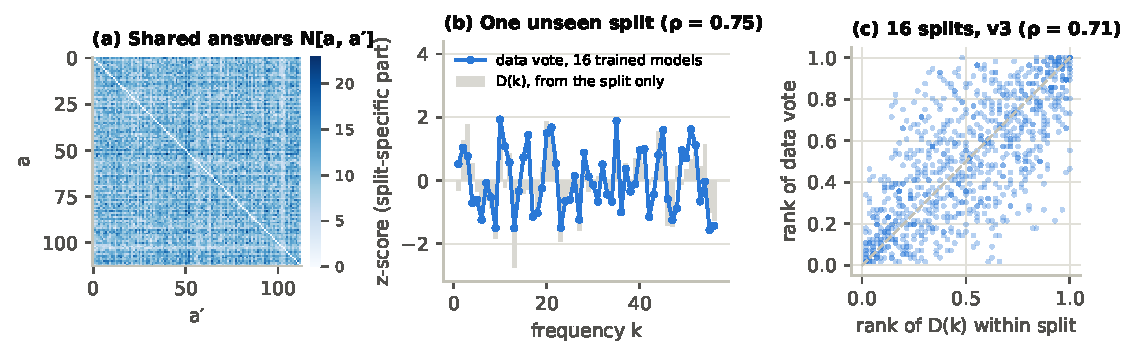
\includegraphics[width=\linewidth]{figures/fig2_dk.pdf}
\caption{\textbf{The shared-answer statistic.} (a)~$N[a,a']$ for one split (diagonal removed). (b)~For a split never used
before: \Dk\ (bars, computed from the list of training pairs) and the data vote measured from 16 trained models (line),
both as split-specific $z$-scores. (c)~All 16 v3 splits, ranks within split. Pre-registered P1: $\rho=0.71$.}
\label{fig:dk}
\end{figure}

\subsection{Why \Dk\ works}
\label{sec:why}
At initialisation the logits are nearly uniform, so the cross-entropy gradient on the embedding of token $a$ is dominated
by $-\sum_{b:(a,b)\in\mathcal{T}} r_{a+b}$, where $r_c$ is the direction (through OV, MLP and $W_U$) that raises logit $c$.
For random weights in $d=128$ these directions are nearly orthogonal, so in the first steps
\begin{equation}
  \Delta E_a \;\approx\; \eta\sum_c N_1[a,c]\, r_c,\qquad \Delta E\,\Delta E^\top \approx \eta^2\|r\|^2 N,
\end{equation}
where $N_1[a,c]=1$ if $(a,c-a)\in\mathcal{T}$. The power of $\Delta E$ at frequency $k$ is therefore $\propto\Dk$. This is
the leading term of known analyses~\citep{yao2025probability,wang2026probability,tian2025provable}. What we add is its use
on a \emph{finite} split, where $N$ is not circulant, as a per-frequency predictor.

Two consequences check out (exploratory). First, the relation holds run by run: each run's own early $\Delta E$ spectrum
correlates with its own split's \Dk\ after removing the part shared across splits (mean $\rho=0.34$ at step 10 and
$0.38$ at step 30; all 16 runs positive, minimum $0.18$). It anti-correlates with the other splits' \Dk\ (mean $-0.12$).
Plain SGD gives the same picture (0.37), so this is not an Adam effect. Second, for a random split, \Dk\ is a sum of $p$ independent terms, so its
relative spread across $k$ should be $\approx1/\sqrt{n}$, independent of the training fraction. The observed spread is
0.095--0.099 at four training fractions (prediction 0.094). Across primes and operations it matches within the
pre-registered $\pm25\,\%$ (Fig.~\ref{fig:general}b; G2 \pass).

\subsection{Generalisation}
\label{sec:general}
\Dk\ was fixed at $p=113$ and then tested unchanged (v4) at $p=59$ and $p=97$, for addition and for multiplication in the
discrete-log basis (Table~\ref{tab:general}, Fig.~\ref{fig:general}). All four configurations pass both the rank test
(G1: $\rho>0.3$, $p<0.01$) and the spread test (G2). That the multiplication runs pass indicates the mechanism follows
the group structure, not the token encoding. In the two-layer model (v7, T2) \Dk\ predicts the data vote with
$\rho=0.72$.

\begin{table}[t]\centering\small
\caption{\textbf{Pre-registered generalisation of \Dk} (v4: 8 splits $\times$ 12 inits per configuration, step 100; v7:
8 splits $\times$ 12 inits, step 200). $n$ is the group order. Reliability is the split-half reliability of the data vote.}
\label{tab:general}
\begin{tabular}{@{}lcccccc@{}}\toprule
configuration & $n$ & Spearman(\Dk, vote) & $p$ & spread / $(1/\sqrt n)$ & reliability & verdict \\\midrule
$a+b \bmod 59$ & 59 & 0.645 & $10^{-4}$ & 0.89 & 0.93 & \pass \\
$a\cdot b \bmod 59$ & 58 & 0.739 & $10^{-4}$ & 1.01 & 0.94 & \pass \\
$a+b \bmod 97$ & 97 & 0.673 & $10^{-4}$ & 0.93 & 0.93 & \pass \\
$a\cdot b \bmod 97$ & 96 & 0.690 & $10^{-4}$ & 0.92 & 0.93 & \pass \\
$a+b \bmod 113$, 2-layer (v7) & 113 & 0.718 & $10^{-4}$ & -- & -- & \pass \\\bottomrule
\end{tabular}
\end{table}

\begin{figure}[t]\centering
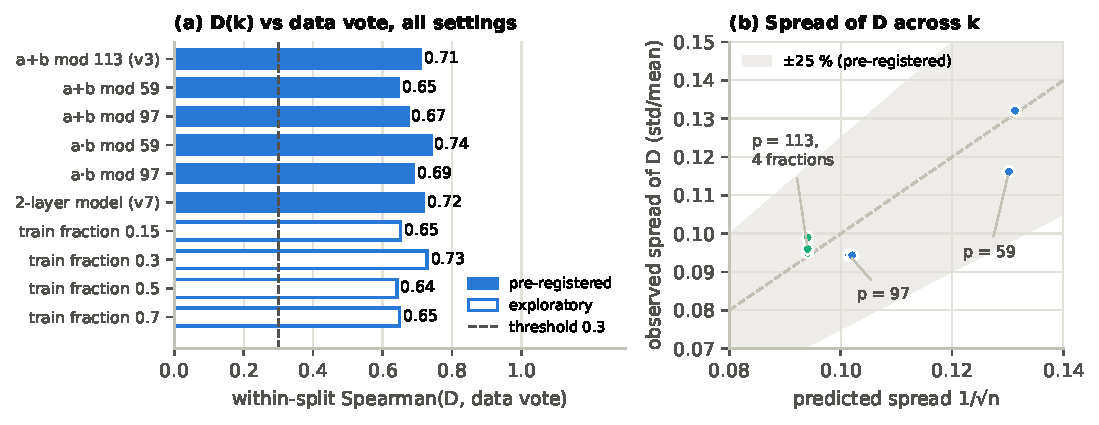
\includegraphics[width=\linewidth]{figures/fig4_generalisation.pdf}
\caption{\textbf{\Dk\ generalises.} (a)~Within-split Spearman between \Dk\ and the data vote in every setting we tested.
Filled bars are pre-registered; outlined bars come from an exploratory training-fraction sweep at $p=113$. (b)~Relative
spread of \Dk\ across frequencies against the random-split prediction $1/\sqrt n$. Blue: v4 configurations
(pre-registered); green: four training fractions at $p=113$.}
\label{fig:general}
\end{figure}

\subsection{Steering: choosing the frequency in advance}
\label{sec:steer}
If \Dk\ captures how the split shapes selection, it should also work as a control. We drew 8 target frequencies at random,
$k^\star\in\{2,17,25,28,33,35,41,43\}$. For each, starting from a random base split, we greedily swapped training pairs
with held-out pairs to raise $J=\log D(k^\star)-\text{mean}_{k\neq k^\star}\log\Dk$ by a gain $g\in\{0,0.15,0.3,0.6,1.0\}$.
No network is involved, and the split size and the per-input and per-answer pair counts are unchanged. At $g=1$, between
412 and 481 of the 3830 training pairs (11--13\,\%) were swapped. We then trained 12 fresh inits on every split (v5) and
repeated the extreme conditions in a two-layer model with fresh inits (v7).

\begin{table}[t]\centering\small
\caption{\textbf{Steering results} (pre-registered). ``Early'': target among the top-3 frequencies of the step-200
spectrum (96 runs per cell). ``Final'': target is a key frequency of the circuit after training (16 runs per cell; up to
10\,000 steps in 1 layer and 15\,000 in 2 layers).}
\label{tab:steer}
\begin{tabular}{@{}llccl@{}}\toprule
model & outcome & original split & steered split ($g=1$) & pre-registered test \\\midrule
1-layer & early & 4\,\% & \textbf{100\,\%} (96/96) & S1 \pass\ ($p=0.004$) \\
1-layer & final circuit & 1/16 & \textbf{16/16} & S3 \pass\ ($p=3\cdot10^{-8}$) \\
2-layer & early & 3\,\% & \textbf{100\,\%} (96/96) & T1 \pass\ ($p=0.004$) \\
2-layer & final circuit & 0/16 & \textbf{15/16} & T3 \pass\ ($p=3\cdot10^{-8}$) \\\bottomrule
\end{tabular}
\end{table}

\begin{figure}[t]\centering
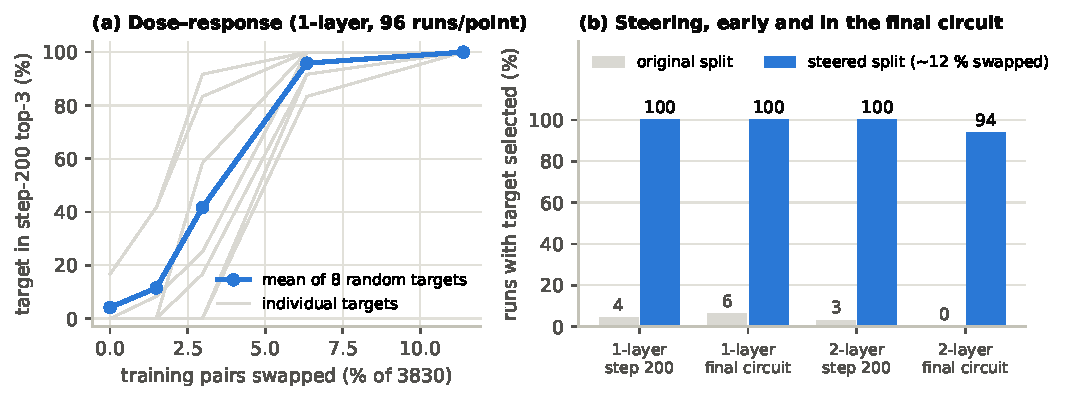
\includegraphics[width=\linewidth]{figures/fig5_steering.pdf}
\caption{\textbf{Steering by editing the split.} (a)~Dose--response in the one-layer model: the fraction of runs in which
the target is a leading frequency at step 200, against the fraction of training pairs swapped (grey: individual targets;
blue: mean). Pre-registered S2: mean within-target Spearman 0.95. (b)~Original vs.\ steered splits, early and in the final
circuit, for one- and two-layer models.}
\label{fig:steer}
\end{figure}

The effect is large and graded (Table~\ref{tab:steer}, Fig.~\ref{fig:steer}). In the one-layer model the target leads at
step 200 in 4\,\%, 11\,\%, 42\,\%, 96\,\% and 100\,\% of runs as $g$ rises (S2: within-target Spearman 0.95, $p=10^{-4}$,
\pass). After full training, the target is part of the final circuit in all 16 steered runs and in 1 of 16 runs from the
same inits on the original splits (S3 \pass). Steering worked equally well for targets that the initialisation ranked in
the bottom half of its own preference (exploratory: 100\,\% in both halves). The two-layer model reproduces the effect: 3\,\%
$\to$ 100\,\% early, and 0/16 $\to$ 15/16 in the final circuit. The one miss ($k^\star=17$) carries the target in its
block-2 neuron clusters but below the 5\,\% logit threshold. The secondary neuron rule gives 16/16 vs.\ 0/16.

Steering does not damage learning. In one layer, 15 of 16 steered runs grokked within 10\,000 steps (median step 4250),
against 16/16 on the original splits (median 6375). The run that did not grok reached 88\,\% test accuracy. In two layers
all 32 runs grokked, the steered ones earlier (median 4000 vs.\ 5125 steps), with mean final test accuracy $\ge99.7\,\%$
in both arms. One-layer stage B ran 4 runs on CPU and 28 on a GPU, with the same code and hash-verified splits; the
pre-registration did not specify the device.

\subsection{The init side}
\label{sec:init}
At the \texttt{=} position of the one-layer model, the operands enter the residual stream only through the attention OV
map. Grokking builds its features in the MLP, so the amplitude a frequency starts with should be read from the token map
\emph{as seen through OV}, $W_E W_{OV}$, rather than from $W_E$. This is a transformer analogue of the MLP result
of~\citet{ding2024survival}. A frequency-$k$ feature also needs an output factor; for a two-factor feature $u_kv_k$
growing from small initialisation, the escape time scales as $-\log(u_kv_k)$, which suggests the parameter-free
\emph{product rule} $\log P_{\text{in}}(k)+\log P_{\text{out}}(k)$, with $P_{\text{out}}$ the Fourier power of $W_U$ over
answer classes. Both ideas hold in exploratory tests on stored data (Fig.~\ref{fig:init}a, Table~\ref{tab:init}). The OV
readout beats $W_E$ on every data set, and the product rule improves it further. Combined with \Dk, the product rule raises
training-free top-3 hits on the v1 test factorial from 961 to 1008.

\begin{table}[t]\centering\small
\caption{\textbf{Init-side readouts} (exploratory, 1 layer): mean per-init Spearman with the init vote and top-3 hits on
the winners. v1 dev/test: 3072 slots, chance 165; v3: 768 slots, chance 41.}
\label{tab:init}
\begin{tabular}{@{}lcccccc@{}}\toprule
& \multicolumn{2}{c}{v1 dev} & \multicolumn{2}{c}{v1 test} & \multicolumn{2}{c}{v3} \\\cmidrule(lr){2-3}\cmidrule(lr){4-5}\cmidrule(lr){6-7}
readout at initialisation & $\rho$ & hits & $\rho$ & hits & $\rho$ & hits \\\midrule
$W_E$ & 0.67 & 523 & 0.69 & 485 & 0.71 & 132 \\
$W_E W_{OV}$ & 0.77 & 594 & 0.77 & 576 & 0.72 & 154 \\
$W_U$ (over classes) & 0.29 & 330 & 0.26 & 363 & 0.15 & 83 \\
product rule $W_EW_{OV}\times W_U$ & \textbf{0.80} & \textbf{680} & \textbf{0.79} & \textbf{646} & \textbf{0.73} & \textbf{162} \\\midrule
\multicolumn{7}{@{}l}{\emph{combined with \Dk\ (equal-weight $z$-sum):}}\\
$W_EW_{OV}$ + \Dk & & 945 & & 961 & & 230 \\
product rule + \Dk & & \textbf{992} & & \textbf{1008} & & \textbf{234} \\\bottomrule
\end{tabular}
\end{table}

\begin{figure}[t]\centering
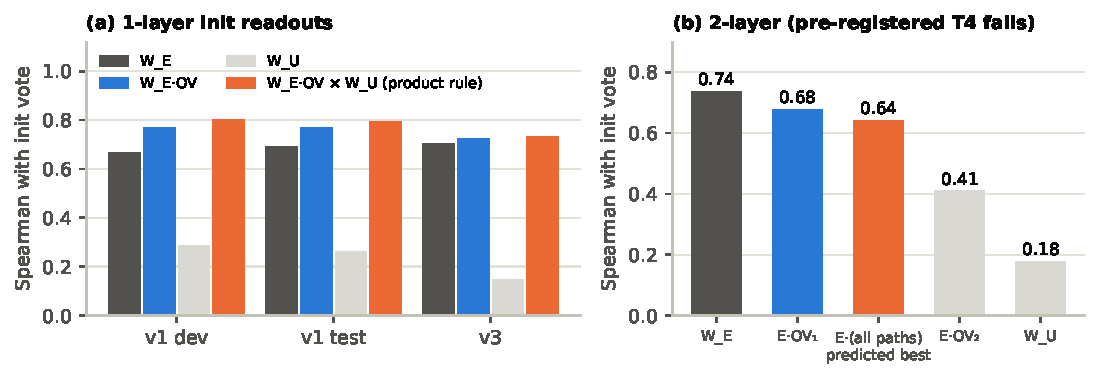
\includegraphics[width=\linewidth]{figures/fig6_init.pdf}
\caption{\textbf{Reading the init vote at initialisation.} (a)~One layer (exploratory): the OV-path spectrum beats the raw
embedding spectrum, and multiplying by the unembedding spectrum helps further. (b)~Two layers (pre-registered T4): we
predicted that the readout through all linear attention paths, $E(OV_1+OV_2+OV_1OV_2)$, would beat $E\,OV_1$. It did not
(0.64 vs.\ 0.68), and the raw embedding was best (0.74).}
\label{fig:init}
\end{figure}

How the init and data terms combine is not settled. The obvious physical model treats the data as extra input power,
$P_{\text{in}}+\gamma\Dk$. Its best $\gamma$ on dev gives 829 hits, far below the equal-weight $z$-sum (945); \Dk\ varies by
only $\sim$10\,\% across $k$, so adding it as power changes little. We suspected that data-driven updates are aligned with
the output pathway while random initial structure is not. The early $\Delta E$ is indeed more aligned with
$W_{OV}W_U$ at each frequency than the initial embedding: mean $|\cos|$ is 0.13--0.16 at step 10, against 0.076--0.080 at
initialisation and 0.078 for random vectors. But the alignment does not track \Dk\ across frequencies
($\rho=-0.08$ to $+0.20$), so it cannot explain the ranking.

For two layers we pre-registered the natural extension (T4). The MLPs now see the operands through both attention layers,
so the readout should use the full linear token map. This failed (Fig.~\ref{fig:init}b). A post-hoc reading is that block-2
attention reads $E$ directly at the operand positions, and block 1 builds features there too, so the one-layer premise no
longer holds. We have not tested this.

\subsection{Training-free prediction}
Combining the two readouts gives a prediction that needs no trained model: z(OV spectrum at init) + z(\Dk). On the v1 test
factorial it reaches 961 top-3 hits, against 576 for the init readout alone, 701 for \Dk\ alone and 1256 for C4, which
needed 64 trained runs per split to estimate the data vote. In the pre-registered v3 test (P2) it gives 230 of 768 against
154 for the init readout alone (chance 41; bootstrap CI of the difference $[28,123]$, \pass). Against the final circuits
of 64 fully trained runs, 43\,\% of its top-3 frequencies are key frequencies (product rule: 45\,\%), against 27\,\% for
the init readout alone and 9\,\% by chance.

\subsection{Failures}
\label{sec:fail}
\begin{figure}[t]\centering
\begin{minipage}[c]{0.44\linewidth}\centering
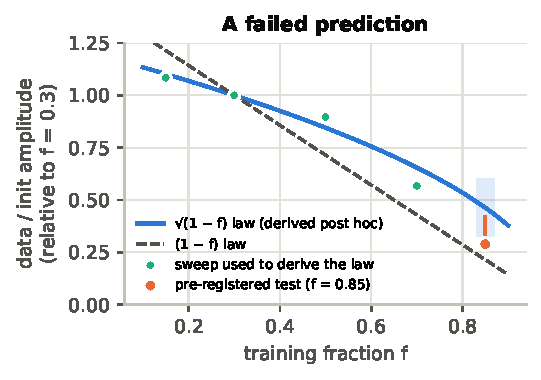
\includegraphics[width=\linewidth]{figures/fig7_fraction.pdf}
\end{minipage}\hfill
\begin{minipage}[c]{0.53\linewidth}
\caption{\textbf{A failed pre-registered prediction (v6).} The data vote weakens as the training fraction $f$ grows. An
energy-fraction argument, derived after seeing the sweep (green), predicts an amplitude ratio $\propto\sqrt{1-f}$. At a
new fraction ($f=0.85$, fresh seeds) the prediction was $0.46$ with a window of $[0.32,0.60]$ (shaded). We observed
$0.29$, so the effect shrinks faster, roughly as $(1-f)^{0.7\text{--}0.8}$. The orange bar is the bootstrap 95\,\% interval
(0.30--0.42), which is biased upward by resampling.}
\label{fig:frac}
\end{minipage}
\end{figure}
We list every pre-registered failure (Table~\ref{tab:prereg}):
\begin{itemize}
\item \textbf{C2:} the simple data statistics we tried before \Dk\ did not transfer to test.
\item \textbf{Proxy validity:} early winners contain only 56.5\,\% of the final keys.
\item \textbf{C6:} internal progress measures predicted grokking time worse than a behavioural baseline (Harrell's $C$:
  0.85 vs.\ 0.92).
\item \textbf{H5:} per-pair influence did not replicate across init groups (2 of 4 splits; criterion 3 of 4), and
  the datamodels predict held-out runs poorly ($R^2\approx0.03$).
\item \textbf{F1 (v6):} the $\sqrt{1-f}$ law (Fig.~\ref{fig:frac}).
\item \textbf{T4 (v7):} the two-layer init readout.
\end{itemize}
Both theoretical failures concern the init side or the relative strength of init and data. Neither concerns the data-side
mechanism itself.

\section{Discussion}
The picture that emerges is simple on the data side. Early training is driven by which answers the inputs share in the
training set. That structure is computable from the split, it is a fixed property of the group operation, and it is
strong enough that editing about one pair in eight overrides the initialisation and decides the final circuit. The same
holds in a second architecture. A finite training set is therefore not an unbiased sample of the full table as far as
representation is concerned: it carries a frequency fingerprint, and the network learns it.

Three implications seem worth stating carefully. \emph{Interpretability:} ``why this circuit and not another'' can have an
answer that lives in the data, computable without the model. \emph{Data design:} in this toy setting, a few hundred
well-chosen examples change which algorithm a network implements while leaving accuracy intact. \emph{Theory:} analyses
that average over the training subset discard a systematic, measurable term. The init side is less settled. The OV-path
argument and the product rule work in one layer, but the relative weight of init and data has not been derived, and the
two-layer extension failed.

\section{Limitations}
\begin{itemize}
\item All models are small (one or two layers, $d=128$), all tasks are modular arithmetic with $p\le113$, and nearly
  all runs use one optimiser setting at $f=0.3$. Whether data-composition steering of learned algorithms exists beyond
  group tasks is open.
\item Early ``winners'' and final circuits overlap only partly. We tested steering on both, but the final-circuit tests use
  32 runs per architecture.
\item The init-side theory is partial and two of its pre-registered predictions failed. The weighting of init and data is
  empirical.
\item Several analyses are exploratory and labelled as such; the derivation of \Dk\ is an approximation, not a theorem.
\item In v7 a pipeline smoke test used a subset of the confirmatory seeds after registration; we disclose this in the
  repository. Nothing was changed after seeing it.
\item The literature search was done with automated tools and may be incomplete.
\item One AI system designed, ran and analysed these experiments. Pre-registration and released code are meant to make
  them checkable, but no independent replication exists yet.
\end{itemize}

\section{Contribution statement and reproducibility}
\label{sec:contrib}
Claude (Anthropic, \texttt{claude-opus-5-5}) chose the research question, designed every experiment and pre-registration,
wrote all code, analysed the results, searched the literature and wrote this paper, in a long conversation with Seungho Yu.
Seungho Yu started the project, asked Claude to pursue a question of its own choosing, made the decisions about
compute and publication, and ran the Kaggle GPU jobs. Where a venue does not allow an AI system as an author, Seungho Yu
is the responsible author and this statement describes the division of work.

The repository contains the library (\texttt{src/freqsel}), the code of every stage, all raw results and the pre-registration
texts with a hash verifier. A script recomputes every number in this paper from the stored results in seconds
(\texttt{scripts/reproduce\_claims.py}), and another regenerates every figure (\texttt{paper/make\_figures.py}). The GPU
stages run on a free Kaggle T4.

\bibliographystyle{plainnat}
\bibliography{references}

\clearpage
\appendix
\section{All pre-registered tests}
\begin{table}[!htbp]\centering\footnotesize
\caption{\textbf{Every pre-registered test and its outcome.} Hashes are SHA-256 of the registration text (first 8 hex digits).}
\label{tab:prereg}
\begin{tabularx}{\linewidth}{@{}l l X l@{}}\toprule
stage (hash) & test & criterion $\to$ result & verdict \\\midrule
v1 (\texttt{1034f794}) & C1 & init+data beats each alone (CI$>0$) $\to$ 1265 vs 655 / 959 & \pass \\
 & C2 & dev-selected simple statistic predicts test vote $\to$ no & \fail \\
 & C3 & removing top datamodel pairs lowers $k^\star$, Holm $p<0.01$ $\to$ $p=0.0002$ (both splits) & \pass \\
 & C4 & OV-path + data vote beats OV path $\to$ 1256 vs 576 & \pass \\
 & C5 & median commitment step $\le5\,\%$ of median grokking step $\to$ 2.3\,\% (base), 2.5\,\% (MLP); subtraction not testable (5/16 grokked) & \pass \\
 & C6 & internal measures beat behavioural baseline for grokking time $\to$ $C$ 0.85 vs 0.92 & \fail \\
 & R1 & OV path at init above chance, $p<10^{-3}$ $\to$ 576 vs 165 & \pass \\
 & proxy$^\dagger$ & step-500 winners contain $\ge75\,\%$ of final keys $\to$ 56.5\,\% & \fail \\
v2 (\texttt{9177a4a9}) & H1 & vote persists with shuffled labels ($p<0.01$) $\to$ 0.04, $p=0.048$ & \fail \\
 & H2 & shift relabelling keeps the vote $\to$ 0.955 & \pass \\
 & H3 & vote persists for subtraction on the same pairs $\to$ 0.006 & \fail \\
 & H4 & MLP-only model keeps the vote $\to$ 0.69 & \pass \\
 & H5 & per-pair influence agrees across 2 init groups in $\ge3/4$ splits $\to$ 2/4 & \fail \\
v3 (\texttt{8292aeae}) & P1 & Spearman(\Dk, vote) $>0.5$, $p<10^{-3}$ $\to$ 0.709 & \pass \\
 & P2 & OV + \Dk\ beats OV, CI$>0$ $\to$ 230 vs 154, $[28,123]$ & \pass \\
v4 (\texttt{95c74926}) & G1 & $\rho>0.3$, $p<0.01$ in all 4 configs $\to$ 0.65--0.74 & \pass \\
 & G2 & spread within $\pm25\,\%$ of $1/\sqrt n$ $\to$ ratios 0.89--1.01 & \pass \\
v5 (\texttt{8f973240}) & S1 & steered early rate $\ge0.5$ and $>$ original $\to$ 100\,\% vs 4\,\% & \pass \\
 & S2 & dose--response Spearman $>0.5$ $\to$ 0.95 & \pass \\
 & S3 & final-circuit rate steered $>$ original, $\ge50\,\%$ $\to$ 16/16 vs 1/16 & \pass \\
v6 (\texttt{2f243aaa}) & F1 & $R\in[0.324,0.602]$ $\to$ 0.289 & \fail \\
v7 (\texttt{318f50ae}) & T1 & 2-layer early steering $\to$ 100\,\% vs 3\,\% & \pass \\
 & T2 & 2-layer \Dk\ $\rho>0.3$ $\to$ 0.72 & \pass \\
 & T3 & 2-layer final circuit $\to$ 15/16 vs 0/16 & \pass \\
 & T4 & all-paths readout beats $E\,OV_1$ $\to$ 0.64 vs 0.68 & \fail \\\bottomrule
\end{tabularx}
\end{table}
$^\dagger$The proxy threshold was fixed in the v1 analysis code before the run, not in the registration text.
H1 and H3 were registered as hypotheses that the vote would \emph{persist} when only the inputs are kept (shuffled
labels) or the task is changed (subtraction). Their failure is informative: the vote is set by the equations, that is, by
the group structure of input--answer pairs, not by which inputs are present.

\section{Seeds and settings}
Dev seeds: inits and splits $0..31$ (v1 dev). Test: $1000..1031$ (v1 test); $5000..5015$/$6000..6015$ (v3 splits/inits);
$8000..8007$/$8100..8111$ (v4); $9500..9507$ base splits and $9600..9611$ inits (v5); $7600..7607$/$7700..7711$ (v6);
$9800..9811$ (v7); 2-layer pilot $9990,9991$. One-layer stage B: 10\,000 steps; two-layer stage B: up to 15\,000 steps,
stopping 2000 steps after all runs in a batch reached 90\,\% test accuracy. Test accuracy was evaluated every 250 steps.
\end{document}
